\section{Wikidata}

Wikidata is the free and open knowledge base by the Wikimedia movement, which collects multilingual structured data in one central place and makes it publicly available under CC0, a public domain dedication. \footnote{\href{https://creativecommons.org/publicdomain/zero/1.0/}{https://creativecommons.org/publicdomain/zero/1.0/}} Similar to Wikipedia it can be edited by anyone. Wikidata collects data on different topics like people, places, events and many more in so called \textit{items}.
\begin{figure}[H]
	\centering
	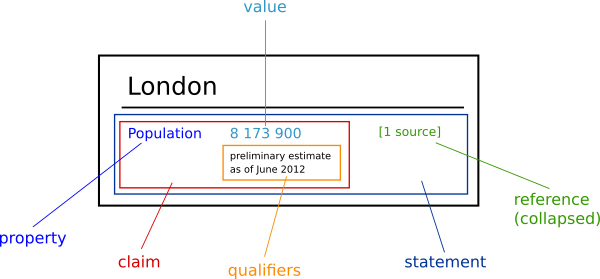
\includegraphics[width=\textwidth]{diagrams/Wikidata_statement.png}
	\caption{Example for Wikidata item London}
	\label{diagramWikidataStatement}
\end{figure}
%\footnote{\href{https://commons.wikimedia.org/wiki/File:WikidataTermDescriptorDiagram.png}{Reference}}
Every item has an identifier, starting with the letter ``Q'' followed by a number unique to the item. Therefore it is clearly identifiable and not depending on labels in natural language, which may change or be ambiguous. Additionally this offers the possibility of referring to the same item in multiple languages by having only one ID. \\
Statements contain a \textit{property}, which is the core part and indicating, what kind of statement is made, and references to prove th claim. One or more values are attached to this property. For example, a claim for a city could be the property \textit{``Population'' (P1082)} with the respective number of inhabitants. There can be multiple values for population of different years, differentiated by \textit{qualifiers}. To identify the important and most recent data, the values can be marked as preferred, normal and deprecated. If the claim has references proving the facts stated, it's a statement. \\
Data types for the properties are items, string, quantity, names of Wikimedia Commons files, geo coordinate, time, URL,  and in the near future also identifier of other databases like VIAF. \\
Properties and items are \textit{entities} in Wikidata. \\
Items can have \textit{sitelinks}. Sitelinks are links to Wikipedia or other Wikimedia projects such as Wikivoyage.
As mentioned before, the data is published under CC-0 and therefore free to anyone to copy, use and distribute.
The aim is not only to have a knowledge base that supports Wikipedia but can also be used in other contexts in the semantic web. Therefore, Wikidata offers an API as well as a SPARQL endpoint. Additionally, the data can be downloaded as a full database dump in the formats JSON, XML and RDF. \todo[inline]{Wikidata's connection to Wikipedia}